\subsection{Related Work}
\label{sec:naysayer_related}

 \begin{figure}[tb]
    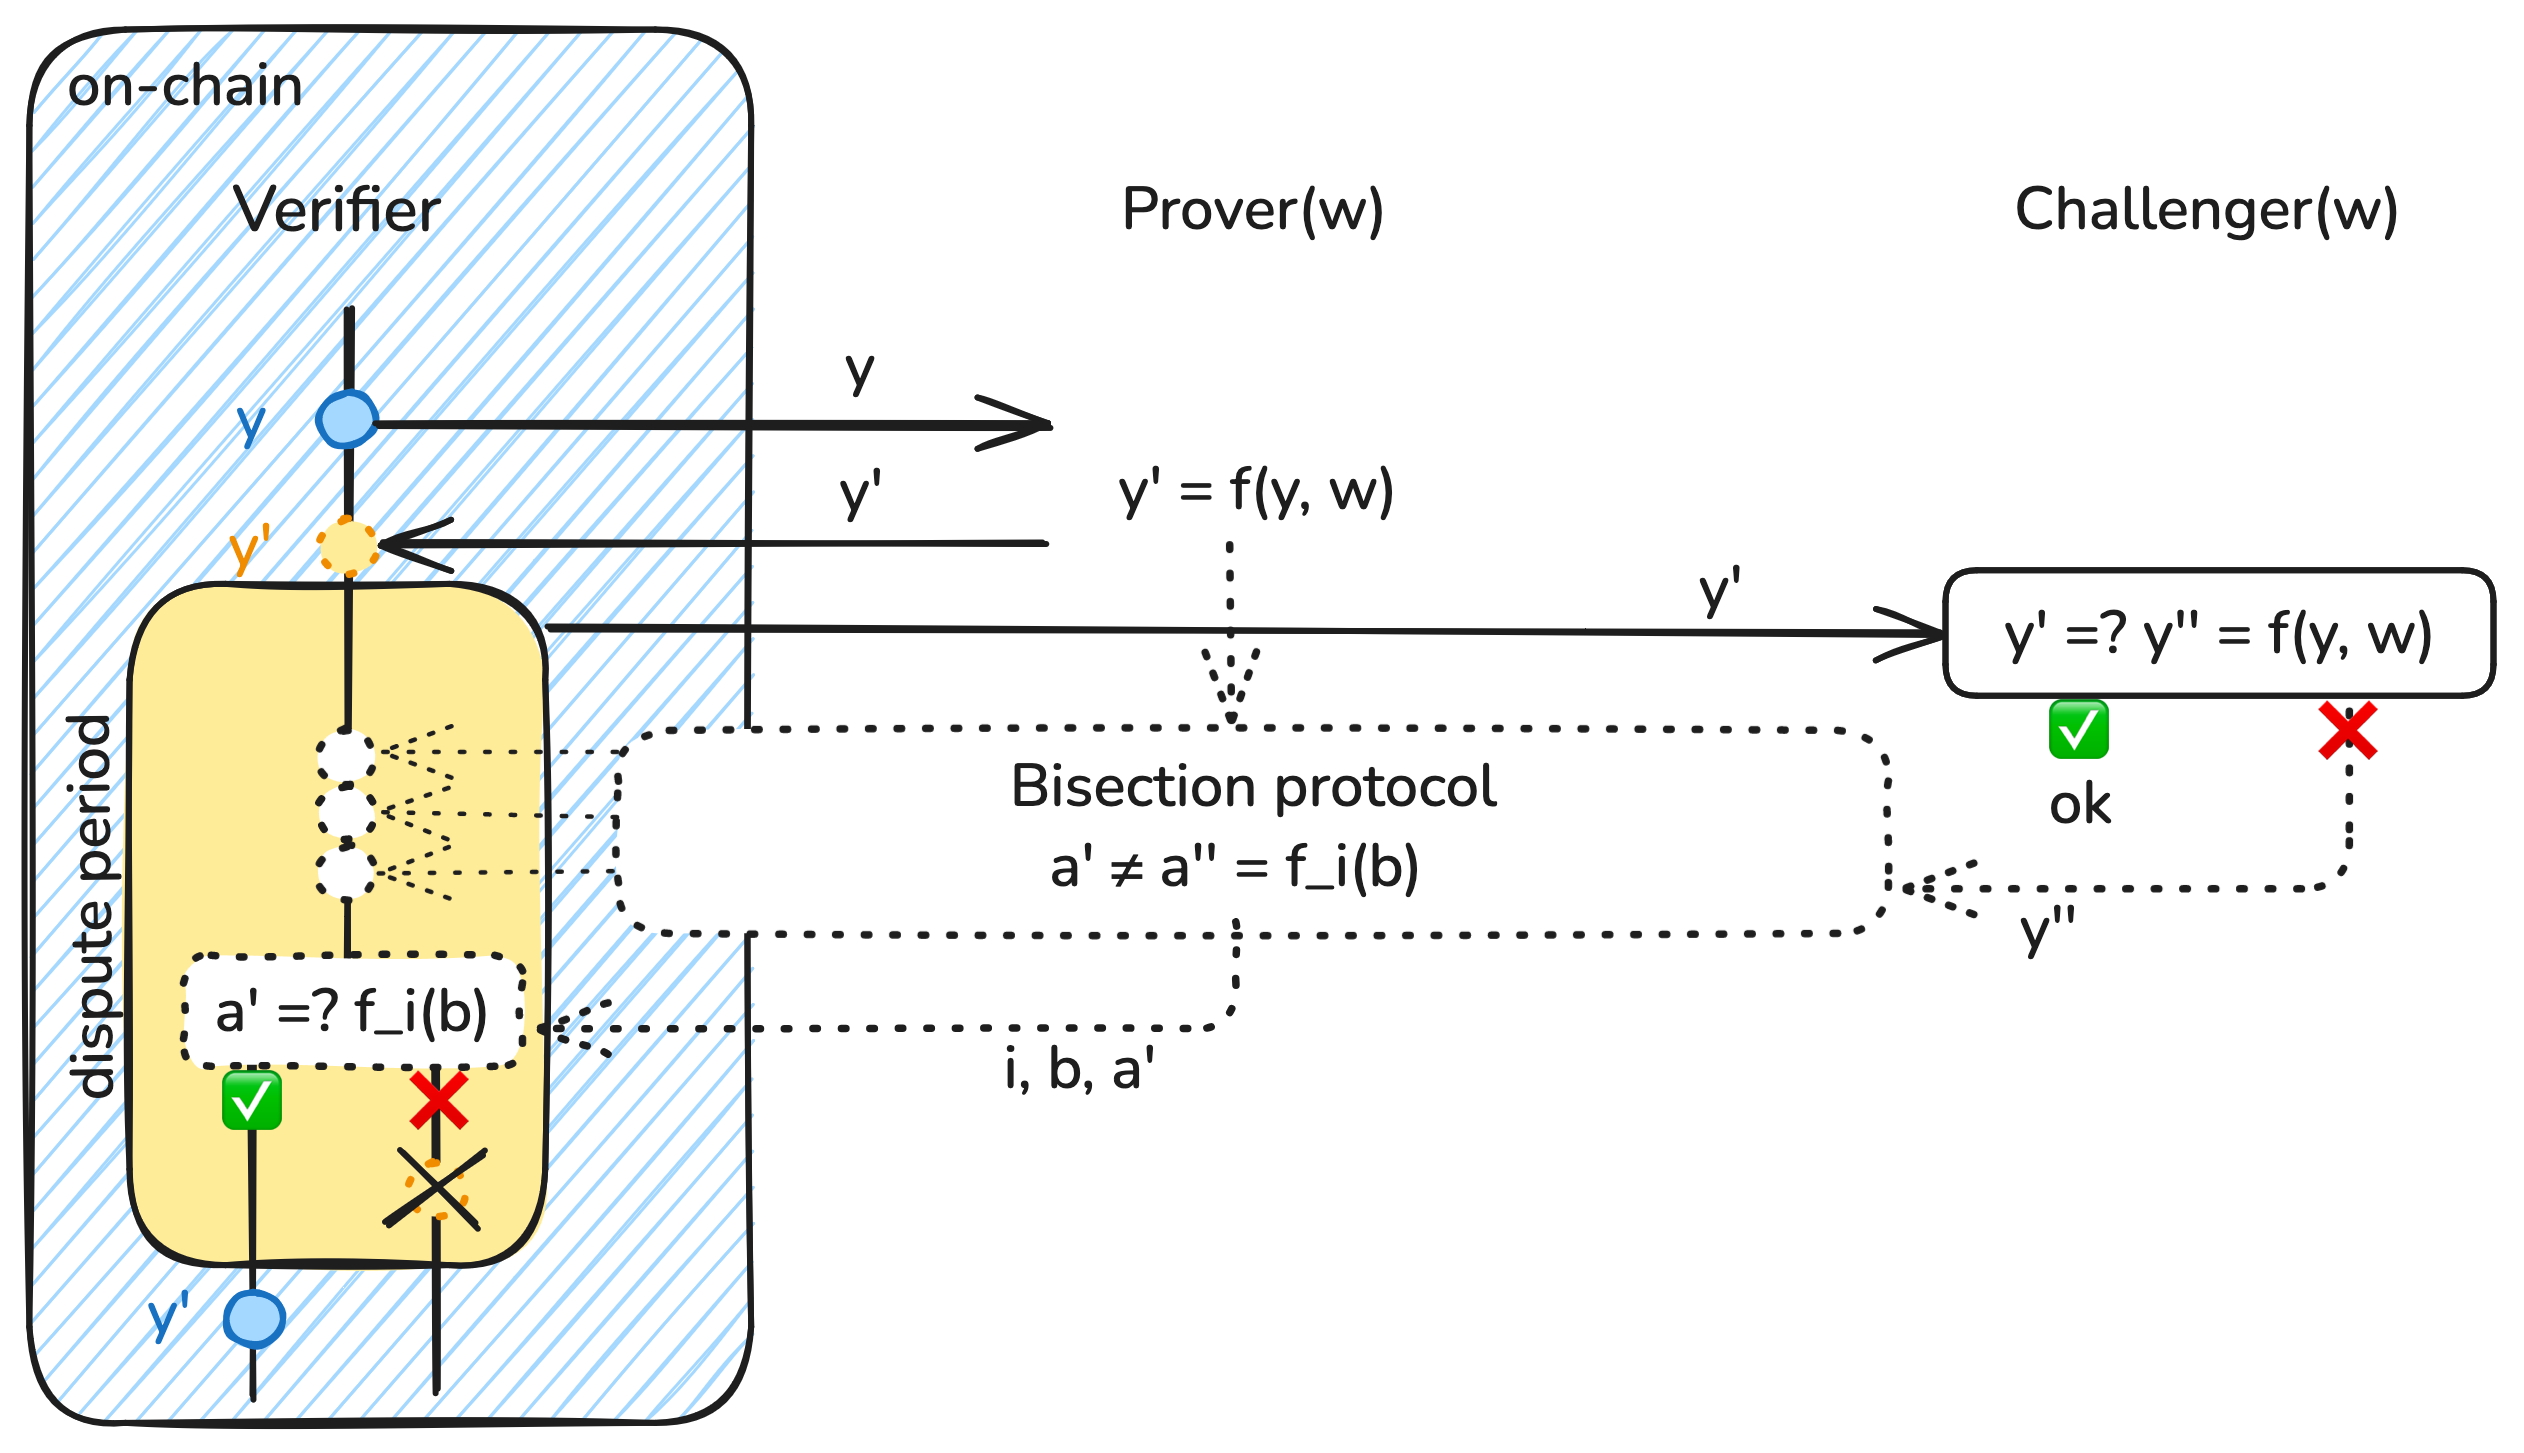
\includegraphics[width=\textwidth]{naysayer/figs/fraud-interactive.png}
    \caption{\textbf{Interactive fraud ``proofs''.} Like naysayer proofs, fraud ``proofs'' make use of challengers and challenge periods. Again, the off-chain ``prover'' computes $y' = f(y, w)$, but without providing any proof of correctness $\pi$. During the challenge period, anyone (with access to $w$, e.g., the batch of transactions) can re-compute $f(y, w)$. If the result $y''$ does not equal $y'$, the party engages in a bisection protocol with the original ``prover'' to narrow the disagreement to a single step of the computation $f_i(b)$. The defender and challenger submit their respective one-step results $a' \neq a''$ to the on-chain verifier, who re-executes $f_i(b)$ on-chain. Based on the result, it may reject the original claim $y'$. If the challenge period elapses without any successful fraud proofs, $y'$ is accepted.}
    \label{fig:fraud-interactive}
 \end{figure}

 \begin{figure}[tbh]
    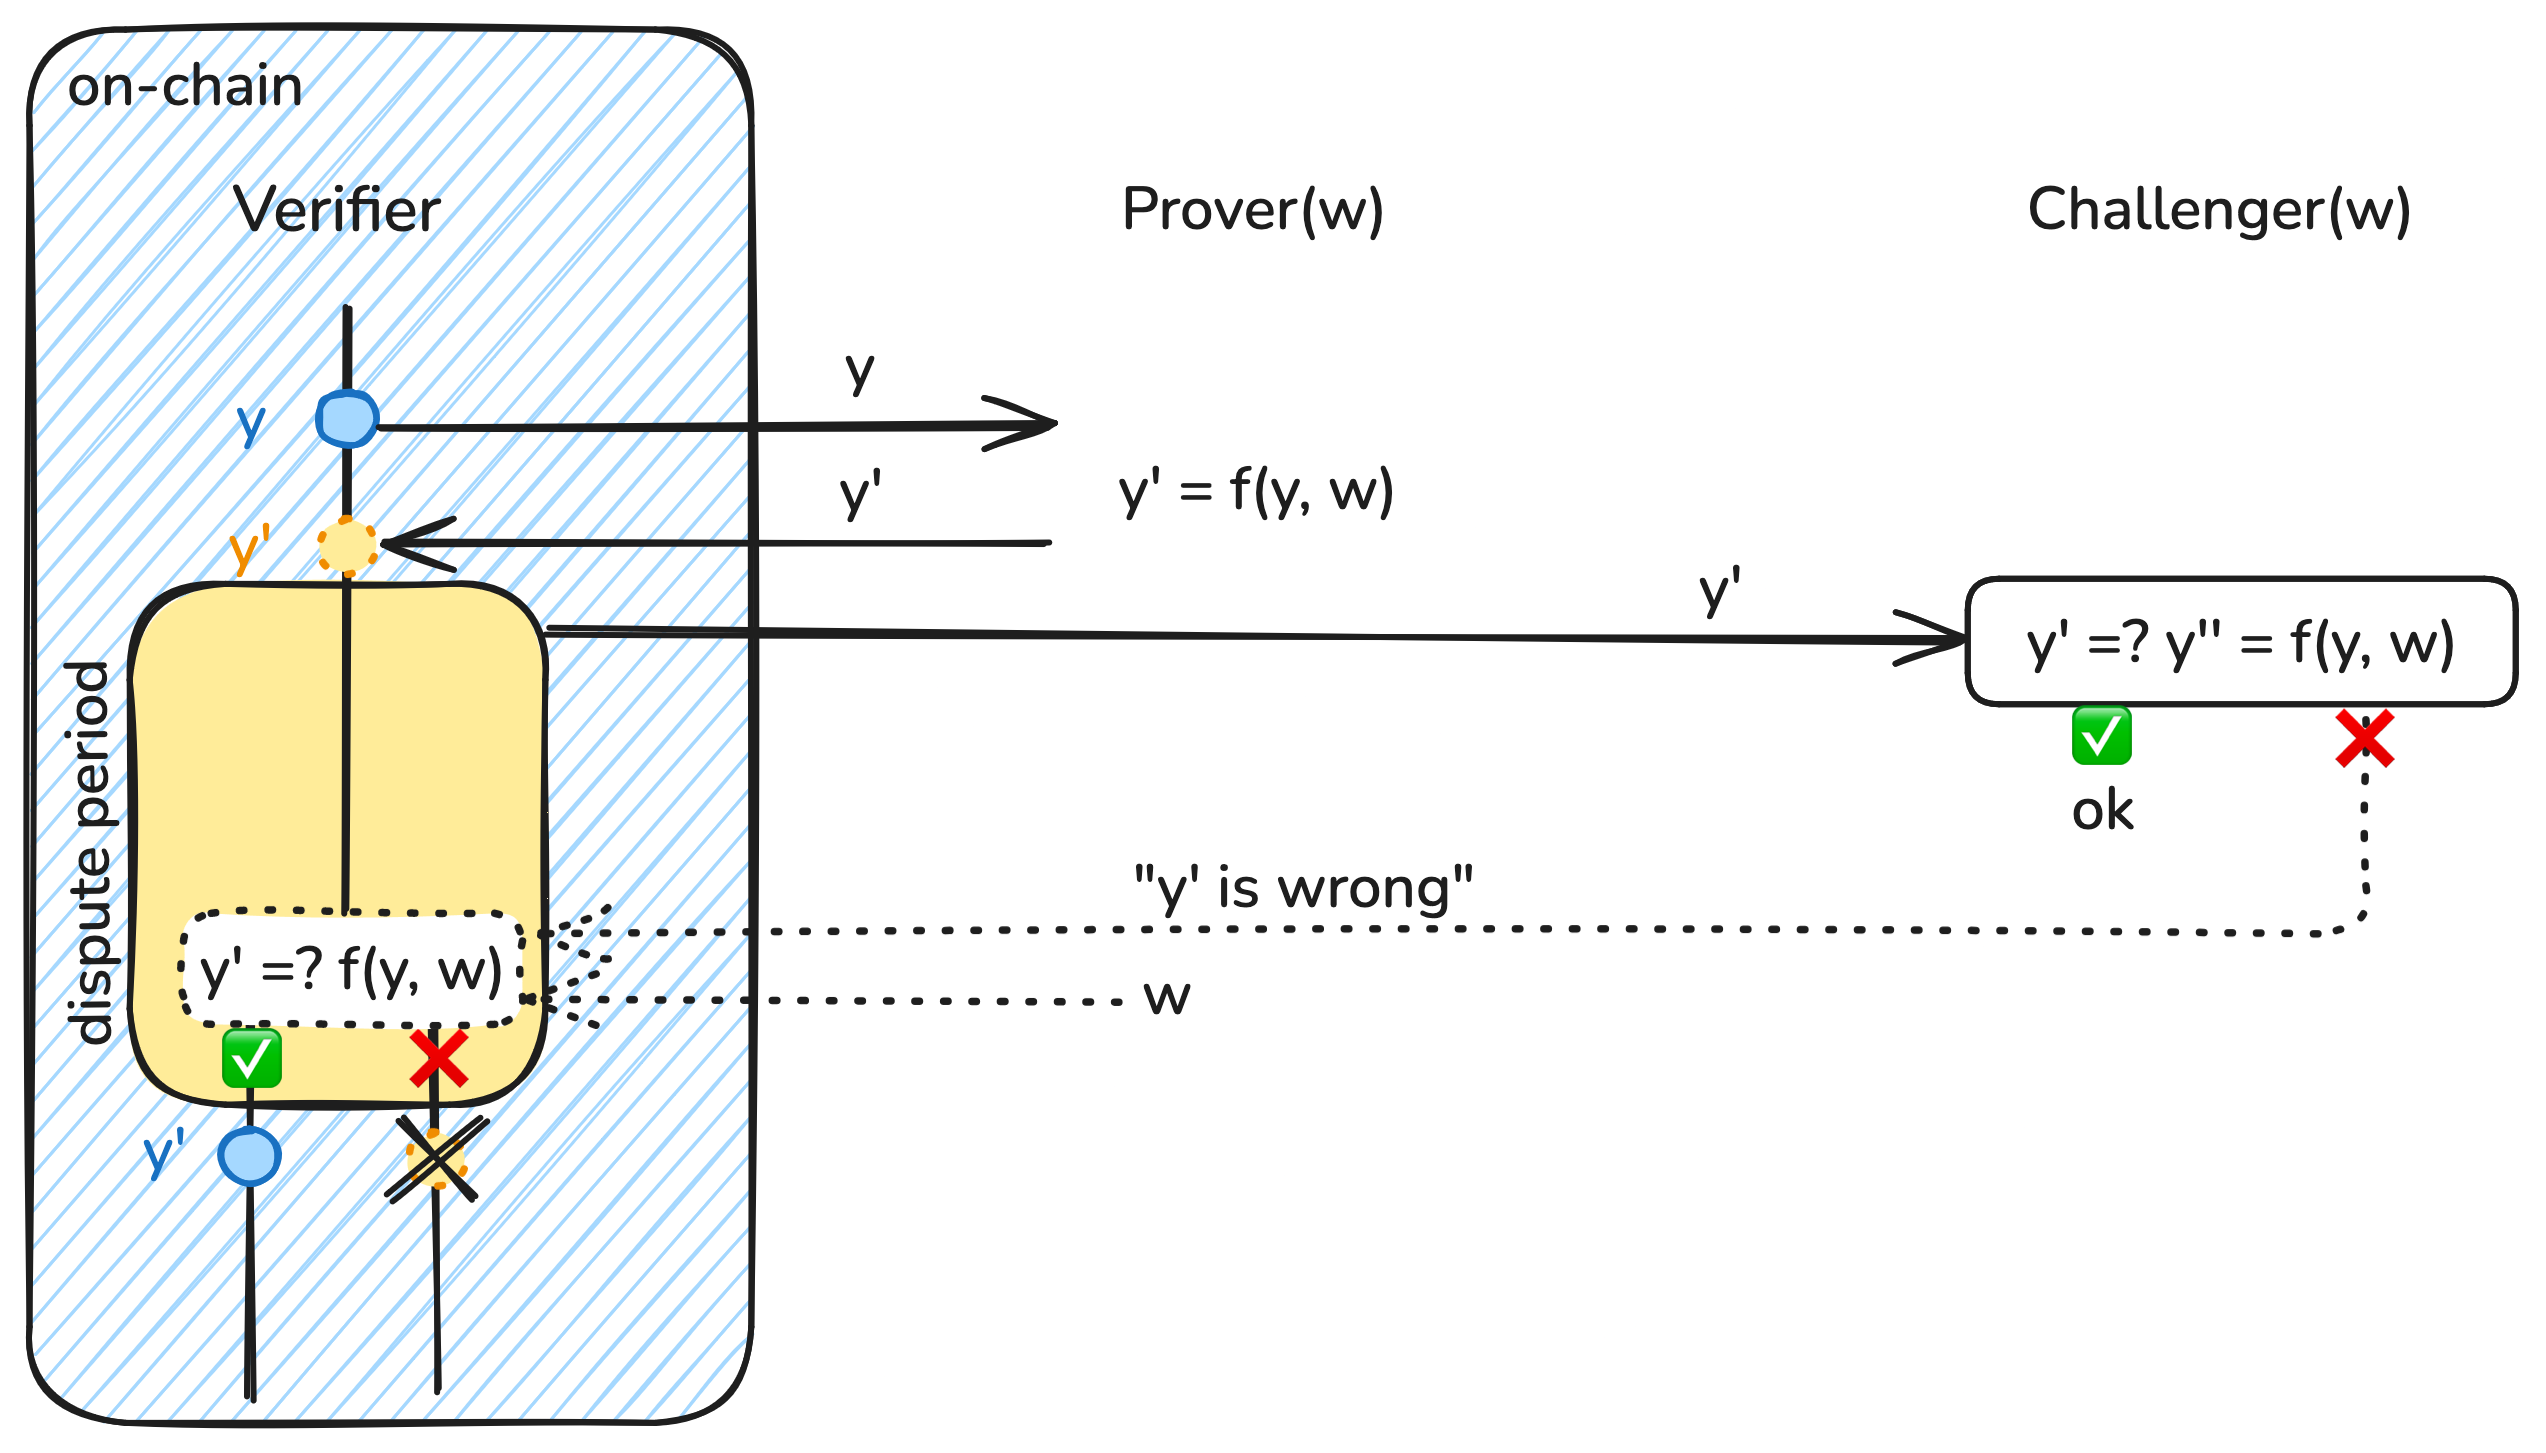
\includegraphics[width=\textwidth]{naysayer/figs/fraud-NI.png}
    \caption{\textbf{Non-interactive fraud ``proofs''.} The non-interactive version functions similarly, except that there is no bisection game. Instead, the on-chain verifier simply re-executes the entire computation $f(y, w)$ on-chain to decide whether or not to reject $y'$. Again, if the challenge period elapses without any challenges, $y'$ is accepted.}
    \label{fig:fraud-NI}
 \end{figure}

A concept related to the naysayer paradigm is \emph{refereed delegation}~\cite{STOC:FeiKil97}. The idea has found widespread adoption~\cite{ARXIV:TeuRei19,USENIX:KGCWF18} under the name ``fraud proofs'' or ``fault proofs'' and is the core idea behind \emph{optimistic rollups} \cite{ethereum_optimistic,arbitrum_nitro,optimism_rollup}. In classic refereed delegation, a server can output a heavy computation to two external parties, who independently compute and return the result. If the reported results disagree, the parties engage in a \emph{bisection protocol} which pinpoints the single step of the computation which gave rise to the disagreement by recursively halving the computational trace (essentially performing a binary search). Once the discrepancy has been reduced to a single step of the computation, the original server can re-execute only that step to determine which of the two parties' results is correct. 

In the context of optimistic rollups, a ``prover'' performs the computation off-chain and posts the result on-chain, where it is provisionally accepted. Any party can then challenge the correctness of the result by posting a challenge on-chain and engaging in the bisection protocol with the prover via on-chain messages (\Cref{fig:fraud-interactive}). (The term ``fraud proof'' or ``fault proof'' refers to these messages.\footnote{Despite the name, this is not actually a proof system, nor does it depend on any proof system.}) Once the problematic step is identified, it is re-executed on-chain to resolve the dispute. A dispute can also be resolved \emph{non-interactively} by re-running the entire computation on-chain in the event of a dispute (\Cref{fig:fraud-NI}), an approach initially taken by Optimism~\cite{optimism_v1,buckland_fraudproofs}.
If no one challenges the prover's result before the end of the \emph{challenge period} (typically 7 days~\cite{why7days}), it is accepted and irreversibly commited on the layer-1 chain.

% The fraud proof design pattern has been applied in an application-specific way in many blockchain applications besides optimistic rollups, including the Lightning Network~\cite{PooDry16}, Plasma~\cite{PooBut17}, cryptocurrency mixers~\cite{EPRINT:SNBB19}, and distributed key generation~\cite{EPRINT:SJSW19}. 

The naysayer approach offers significant speedups for the challenger over fraud proofs, since for succinct proof systems, verification is much more efficient than the original computation. 
Notice that there is a slight semantic difference between fraud proofs and naysayer proofs: A fraud proof challenges the correctness of the prover's \emph{computation}, and thus can definitively show that the computation output is incorrect. In contrast, a naysayer proof challenges the correctness of the \emph{accompanying proof}, and can therefore only show that the proof is invalid---the computation itself may still have been correct. In practice, there is no reason for this distinction to come up: a prover who performs the computation honestly has no incentive to attach an incorrect proof, since that would mean it wasted computational power to compute the result, but would forfeit the reward (and likely incur some additional penalty).

%Commented out for flow and space
%To improve usability and modularity, researchers have even suggested using succinct proofs of the disputed computation or computation step, replacing the potentially costly on-chain re-execution with proof verification~\cite{buckland_fraudproofs}.

% https://www.alchemy.com/overviews/optimistic-rollups

\begin{table}[t]
    \setlength\tabcolsep{0.5em}
    \centering
    \makebox[\linewidth]{
    \begin{tabular}{lcccc}
    \toprule
                                   & VC       & fraud proof       & fraud proof       & naysayer proof \\
                                   &           &   (interactive)   & (non-interactive) &                \\\midrule
        No optimistic assumption   & \yes      & \no               & \no               & \no            \\
        Non-interactive            & \yes      & \no               & \yes              & \yes           \\
        Off-chain $f$  & \yes       & \yes              & \halfcirc             & \yes           \\
        Off-chain $\Pi.\vrfy$  & \no       & -             & -            & \yes           \\
        Witness-independent challenge& \yes    & \no              & \no               & \yes           \\
        Witness-independent resolution& \yes    & \halfcirc              & \no               & \yes           \\
        No $\Pi.\prove$     & \no       & \yes             & \yes              & \no\\
        \bottomrule
    \end{tabular}}
    \caption{Trade-offs between VC, fraud proofs, and naysayer proofs.}
    \label{tab:comparison}
\end{table}

We compare classic verifiable computation, fraud proofs, and our naysayer proofs in \Cref{tab:comparison}. We discuss the main differences in more detail below.

\begin{description}
   \item[\textbf{Assumptions.}]
   Both fraud proofs and naysayer proofs work under an optimistic assumption, meaning a computation is accepted as correct unless some party challenges it. This requires assuming that at least one honest party is present to challenge any incorrect results. This party must also be \emph{able} to submit a challenge, meaning we rely on the censorship-resistance of the underlying blockchain and assume new messages are added within some known, bounded delay. VC does not rely on these assumptions since every computation is checked at the time the result is submitted. It is well known that this leads to the faster on-chain finality of zk-rollups, which use the VC paradigm and thus do not require a challenge period.
   
   \item[\textbf{On-chain interaction.}]
   Except for the interactive version of fraud proofs, all of the approaches require only a single message from the (off-chain) prover or challenger to the (on-chain) verifier. Optimistic rollups almost universally employ interactive fraud proofs, requiring multiple on-chain messages in case of a dispute. This means the challenge period must be long enough to ensure that all the messages of the bisection protocol can be posted on-chain, even in the presence of some fraction of malicious consensus nodes who delay inclusion of the challenger's (or prover's) messages. We conjecture that by virtue of having a non-interactive challenge phase, naysayer proofs (and non-interactive fraud proofs) admit a shorter challenge period. Furthermore, the challenge period must also be long enough to accommodate the challenge resolution protocol to run on-chain. Thus, naysayer proofs should have an advantage even over non-interactive fraud proofs, since for all practical use cases, the on-chain resolution of the former (verifying a naysayer proof) will always be faster than re-computing the function $f$ on-chain.
    
   \item[\textbf{On-chain computation \& witnesses.}]
   As is their goal, none of the approaches require running the original computation $f$ on-chain, except for non-interactive fraud proofs in the (rare) case of a dispute. 
   Compared to VC, fraud proofs and naysayer proofs do not require running proof verification on-chain (fraud proofs do not use a proof system at all).
   However, fraud proofs require the full computation input (including any off-chain input $\witness$, which we refer to as the witness) to be available to potential challengers and at least in part to the verifier.
   % To resolve such a dispute, however, fraud proofs do require on-chain access to (part of) the auxiliary information $w$ used by the prover to compute $y$ (we refer to $w$ as the ``witness'').
   Neither VC nor naysayer proofs require this information to verify the correctness of the output $y'$: they use only the statement and proof, which are already available on-chain.
   % Hence, naysayer proofs work naturally with zero-knowledge proofs.
   % This can also lead to crucial savings if the witness is very large %as in many cases, the witness is extremely large and, therefore, costly to store on-chain 
   % (e.g., transaction data for a rollup).

   \item[\textbf{Underlying proof system.}]
   Finally, a major advantage of fraud proofs is that they do not use any proof system at all. This makes them much easier to implement and deploy. VC and naysayer proofs, on the other hand, require computing a succinct proof, which is costly both in terms of implementation complexity and prover runtime. %This allows their verifiers and challengers to inherit performance advantages directly from succinct proof systems.
   However, the design and efficiency of the bisection protocol can depend significantly on the programming model used~\cite{USENIX:KGCWF18} and the particular function $f$ being computed~\cite{PooDry16,PooBut17,EPRINT:SNBB19,EPRINT:SJSW19}.
   We thus view naysayer proofs as a drop-in replacement for the many application-specific fault proofs, offering an alternative which is both more general and more efficient.
\end{description}